\documentclass{article}

% Language setting
\usepackage[brazil]{babel}

% Set page size and margins
% Replace `letterpaper' with `a4paper' for UK/EU standard size
\usepackage[letterpaper,top=2cm,bottom=2cm,left=3cm,right=3cm,marginparwidth=1.75cm]{geometry}

% Useful packages
\usepackage{mathtools}
\usepackage{amsfonts}
\usepackage{graphicx}
\usepackage[colorlinks=true, allcolors=blue]{hyperref}

\title{Projeto X: Nome do Projeto}

\author{
    \begin{tabular}{ll}
        Nome 1 & RA:\,123456 \\
        Nome 2 & RA:\,123456  
    \end{tabular}
}

\date{\today}

\begin{document}
\maketitle

\begin{abstract}
Resumo do projeto e do que foi feito.
\end{abstract}

\section{Introdução}

Sua introdução vai aqui! Basta começar a escrever seu documento e usar o botão Recompilar para ver a visualização do PDF atualizada. Exemplos de comandos e recursos comumente usados estão listados abaixo para ajudá-lo a começar.

Uma vez que você esteja familiarizado com o editor, você pode encontrar várias configurações de projeto no menu do Overleaf, acessado através do botão no canto superior esquerdo do editor. Para visualizar tutoriais, guias do usuário e mais documentação, por favor visite a \href{https://www.overleaf.com/learn}{biblioteca de ajuda}.

\section{Alguns exemplos para começar}

\subsection{Como criar Seções e Subseções}

Basta usar os comandos de \texttt{section} e \texttt{subsection}, como neste documento de exemplo! Toda a formatação e numeração são tratadas automaticamente.

\subsection{Como incluir Figuras}

Primeiro, você deve fazer o upload do arquivo de imagem do seu computador usando o link de upload no menu de árvore de arquivos. Em seguida, use o comando \texttt{includegraphics} para incluí-la no seu documento. Use o ambiente figure e o comando caption para adicionar um número e uma legenda à sua figura. Veja o código para a Figura \ref{fig:frog} nesta seção como um exemplo.

Note que sua figura será automaticamente colocada no lugar mais apropriado, considerando o texto ao redor e levando em conta outras figuras ou tabelas que possam estar próximas. Você pode encontrar mais informações sobre como adicionar imagens aos seus documentos neste artigo de ajuda sobre \href{https://www.overleaf.com/learn/how-to/Including_images_on_Overleaf}{inclusão de imagens no Overleaf}.

\begin{figure}
\centering
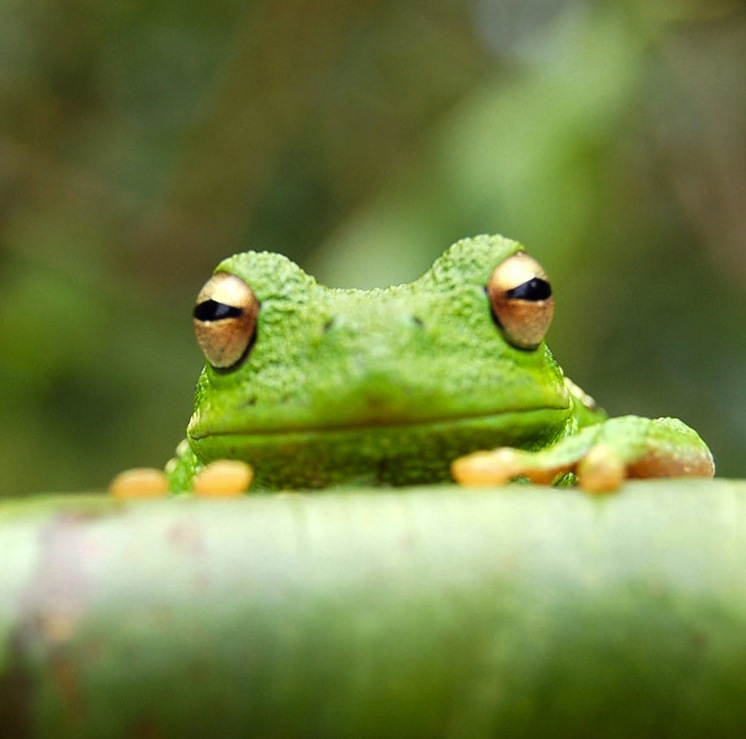
\includegraphics[width=0.25\linewidth]{frog.jpg}
\caption{\label{fig:frog}Este sapo foi carregado através do menu da árvore de arquivos.}
\end{figure}

\subsection{Como adicionar Tabelas}

Use os ambientes \texttt{table} e \texttt{tabular} para tabelas básicas --- veja a Tabela~\ref{tab:widgets}, por exemplo. Para mais informações, por favor veja este artigo de ajuda sobre \href{https://www.overleaf.com/learn/latex/tables}{tabelas}.
%
Também é possível gerar o código das tabelas utilizando o \href{https://www.tablesgenerator.com/}{Tables Generator}.

\begin{table}
\centering
\begin{tabular}{l|c}
Item & Quantidade \\\hline
Camisas & 42 \\
Calças & 13
\end{tabular}
\caption{\label{tab:widgets}Uma tabela de exemplo.}
\end{table}

\subsection{Como adicionar Listas}

Você pode fazer listas com numeração automática \dots

\begin{enumerate}
    \item Assim,
    \item e assim.
\end{enumerate}
\dots ou pontos \dots
\begin{itemize}
    \item Assim,
    \item e assim.
\end{itemize}

\subsection{Como escrever Equações e Fórmulas}

O \LaTeX{} é excelente para a escrita de fórmulas e equações. Seguem exemplos.\\

Todo número $z\in\mathbb{C}$ pode ser escrito na forma $z = x + iy$ com $x,y\in\mathbb{R}$ e $i$ a unidade imaginária.

Se $|z| < 1$, então
\begin{align}
    S &= \sum_{n=0}^{\infty} z^n \label{eq:soma}\\
      &= \frac{1}{1-z}. \label{eq:resultado}
\end{align}
Ademais, a série da Equação~\eqref{eq:soma} converge absolutamente para a Equação~\eqref{eq:resultado}.\\

Caso você queira algum símbolo específico, utilize o \href{https://detexify.kirelabs.org/classify.html}{Detexify} para encontrá-lo!

\subsection{Como adicionar Citações e uma Lista de Referências}

Você pode modificar o arquivo \verb|.bib| contendo entradas BibTeX, que podem ser diretamente adquiridas do \href{https://scholar.google.com/}{Google Scholar}. Em seguida, você pode citar entradas desse arquivo, por exemplo, \cite{greenwade93}.

Não deixe de citar, por exemplo, algum dos livros \cite{stewart} ou \cite{churchill} no seu relatório!

\subsection{Boa Sorte!}

Esperamos que você ache o \LaTeX{} útil.
%
Não deixe de olhar a \href{https://www.overleaf.com/learn}{biblioteca de ajuda} para mais tutoriais.

\bibliographystyle{ieeetr}
\bibliography{bibliografia}

\end{document}